%\chapter{Ngôn ngữ}
\chapter{Tổng quan}
\label{Chapter1}

Trong chương này, khóa luận sẽ trình bày về động lực nghiên cứu, phát biểu bài toán truy xuất ảnh mặt người, các thách thức và giới hạn trong việc thiết kế mô hình gọn nhẹ. Sau đó sẽ trình bày hướng tiếp cận của khóa luận. Cuối cùng là các đóng góp mà khóa luận mang lại.
\section{Động lực nghiên cứu}
% 1. Giới thiệu về vấn đề thực tế và tầm quan trọng của truy xuất hình ảnh khuôn mặt
Trong thời đại phát triển vượt bậc về công nghệ số như hiện nay, ước tính có từ 5 đến 5.3 tỷ ảnh được đăng tải lên toàn cầu mỗi ngày, tương đương 2 triệu tỷ hình ảnh mỗi năm \cite{omnicore2025instagram}. Việc truy xuất ảnh mặt người đã được áp dụng rộng rãi trên thế giới. Trong an ninh công cộng, công nghệ này giúp giám sát và phát hiện tội phạm trong sân bay, nhà ga hay trên đường phố - điển hình như hệ thống camera giám sát quy mô lớn ở Trung Quốc và Anh. Trong thiết bị cá nhân, việc mở khoá bằng nhận diện khuôn mặt đã trở nên phổ biến, với thống kê hơn 131 triệu người Mỹ đã sử dụng công nghệ này hằng ngày. Trong dịch vụ công và hành chính, nhiều quốc gia (Mỹ, Ấn Độ, Liên Minh Châu Âu) triển khai xác thực danh tính công dân khi sử dụng y tế, bảo hiểm xã hội hoặc bỏ phiếu điện tử, - Việt Nam đã sử dụng VneID để xác thực khuôn mặt khi hành khách có mặt tại Nhà ga T3, sân bay Tân Sơn Nhất, thay cho phương pháp kiểm tra giấy tờ truyền thống. 
Những ứng dụng trên cho thấy nhu cầu truy xuất ảnh mặt người đang xuất hiện hầu hết trên các mặt của đời sống xã hội, từ an ninh quốc gia đến đời sống cá nhân.

% 2. Thống kê về sự phát triển thị trường và quy mô dữ liệu
Theo thống kê, thị trường về thị giác máy tính, nhận diện khuôn mặt được định giá khoảng 9.3 tỷ đô trong năm 2025 và kỳ vọng đạt 32.53 tỷ đô vào năm 2034 với tốc độ tăng trưởng trung bình hằng năm (CAGR) 14,93\% \cite{face-recognition-market}. Hơn 1 tỷ camera giám sát đã được triển khai trên toàn thế giới vào năm 2021 \cite{cnbc2019cameras}. Những con số này cho thấy lượng dữ liệu hình ảnh khuôn mặt cần được xử lý là vô cùng lớn, đặt ra yêu cầu cấp thiết cho các hệ thống truy xuất hiệu quả, chính xác và tiết kiệm tài nguyên.

% 3. Thách thức kỹ thuật hiện tại ở quy mô lớn
Tuy nhiên, các mô hình truy xuất hình ảnh khuôn mặt truyền thống với mạng xương sống (như VGG, Resnet, Inception) và Transformer (như ViT, BEiT) khi huán luyện trên tập dữ liệu hàng triệu đến hàng tỷ khuôn mặt đòi hỏi số phép tính dấu phẩy động (FLOP) cực lớn, thời gian tính toán lâu, tiêu hao năng lượng cao \cite{yang2025hiddenjoules}, đặc biệt khó triển khai trên các thiết bị di động và hệ thống giám sát thời gian thực. 

% 4. Lý do cần mô hình nhẹ và tính cấp thiết của nghiên cứu
Vì vậy, chúng tôi tập trung nghiên cứu mô hình truy xuất ảnh mặt người gọn nhẹ, dùng trong dữ liệu có khả năng mở rộng, giúp giảm tải tính toán nhưng vẫn duy trì độ chính xác cao, áp dụng trên các thiết bị di động. 

\section{Phát biểu bài toán}
Có 3 dạng truy xuất ảnh mặt người đang sử dụng hiện nay. Dạng thứ nhất là truy xuất theo danh tính (Identity-based retrieval), tìm ảnh thuộc cùng một danh tính trong cơ sở dữ liệu. Dạng thứ hai là truy xuất theo độ tương đồng (Similarity-based retrieval), tìm ảnh có độ giống cao nhất với ảnh truy vấn, kết quả có thể cùng hoặc khác danh tinh. Dạng cuối cùng là truy xuất theo đặc trưng (Attribute-based retrieval), tìm ảnh dựa trên các đặc điểm khuôn mặt hoặc đặc trưng phụ như giới tính, tuổi, râu hay phụ kiện.

\begin{figure}[htbp] % hoặc [htbp]
    \centering
    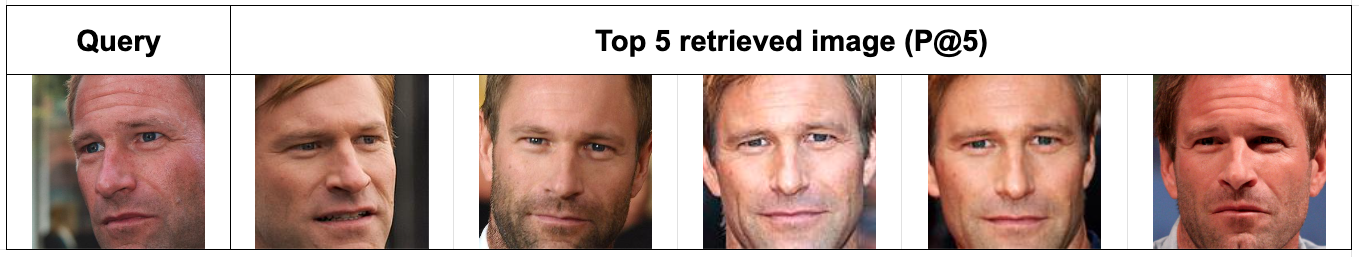
\includegraphics[width=0.8\textwidth]{images/face_retrieval_types.png} 
    \caption{Các dạng truy xuất ảnh mặt người}
    \label{fig:face_retrieval_types}
\end{figure}

\begin{itemize}
    \item[\textbf{Dạng: Truy xuất theo độ tương đồng }]
        \begin{itemize}
            \item[\textbf{Đầu vào:}] Ảnh khuôn mặt truy vấn.
            \item[\textbf{Đầu ra:}] Tập hợp \( K \) hình ảnh có độ tương đồng đặc trưng cao nhất so với ảnh truy vấn, không ràng buộc về danh tính.
        \end{itemize}
\end{itemize}
Đầu vào của các dạng trên đều là ảnh khuôn mặt truy vấn, riêng truy xuất theo đặc trưng cần kèm thêm điều kiện đặc trưng phụ. Đầu ra của dạng thứ nhất: tập hợp K hình ảnh trong cơ sở dữ liệu thuộc cùng danh tính, mức độ giống cao nhất với hình ảnh truy vấn. Đầu ra của dạng thứ hai: tập K hình ảnh có độ tương đồng đặc trưng cao nhất sao với hình ảnh truy vấn, không ràng buộc về danh tính. Đầu ra của dạng thứ ba trả về K hình ảnh vừa có độ tương đồng cao, vừa thoả mãn các đặc trưng phụ đã cho.


\section{Thách thức bài toán}
Việc xây dựng một mô hình truy xuất ảnh mặt người vừa gọn nhẹ vừa có khả năng mở rộng trên tập dữ liệu quy mô lớn phải đối mặt với nhiều thách thức đáng kể. Các thách thức này có thể được phân loại thành ba nhóm chính: thách thức liên quan đến dữ liệu, kiến trúc mô hình xác hiệu suất hệ thống. 

Thứ nhất, về mặt dữ liệu, các hệ thống phải xử lý sự biến đổi phức tạp vốn có trong ảnh mặt người. Một mặt, sự biến đổi trong cùng một danh tính (biến đổi nội lớp) là rất lớn, khi hình ảnh của cùng một các nhân có thể khác biệt đáng kể do sự thay đổi về góc chụp, điều kiện ánh sáng, biểu cảm, quá trình lão hoá, hay sự che khuất bởi các vật thể như khẩu trang, kính râm. Mặt khác, độ tương đồng giữa các biến đổi nội lớp lại có thể rất thấp, khi những cá nhân khác biệt lại sở hữu các đặc điểm khuôn mặt tương tự. Tình trạng này đòi hỏi mô hình phải có khả năng học được một không gian đặc trưng vừa đủ mạnh mẽ để khái quát hoá các biến thể trong cùng một lớp, vừa đủ sức phân biệt để tách bạch các lớp khác nhau. Thêm vào đó, quy mô dữ liệu khổng lồ với hàng triệu đến hàng tỷ hình ảnh làm gia tăng cấp số nhân chi phí tính toán và lưu trữ, đặt ra yêu cầu cấp thiết về hiệu quả trong cả quá trình huấn luyện và truy xuất.

Thứ hai, về kiến trúc mô hình, thách thức cốt lõi nằm ở sự đánh đổi giữa độ chính xác và hiệu quả tính toán. Các mô hình học sâu hiện đại có dung lượng lớn thường đạt độ chính xác cao nhờ khả năng biểu diễn mạnh mẽ, nhưng lại đòi hỏi tài nguyên tính toán khổng lồ, không phù hợp cho việc triển khai trên các thiết bị tài nguyên hạn chế. Do đó, việc thiết kế một kiến trúc mạng gọn nhẹ nhưng vẫn duy trì được khả năng trích xuất đặc trưng có sức phân biệt cao là một bài toán khó. Điều này gắn liền với thách thức về việc học một biểu diễn đặc trưng cô đặc. Việc giảm số chiều của vector đặc trưng là tối quan trọng để tiết kiệm bộ nhớ và tăng tốc độ tìm kiếm, nhưng quá trình này có nguy cơ làm mất mát thông tin nhận dạng quan trọng.

Cuối cùng, về hiệu suất hệ thống, mô hình phải đáp ứng được yêu cầu về tốc độ truy xuất trong thời gian thực. Với có sở dữ liệu quy mô lớn, việc tìm kiếm tuần tự qua toàn bộ dữ liệu là bất khả thi về mặt thời gian. Điều này đòi hỏi phải tích hợp các thuật toán lập chỉ mục và tìm kiếm lân cận gần đúng hiệu quả. Hơn nữa, mục tiêu cuối cùng là triển khai trên các thiết bị biên như điện thoại di động hay camera thông minh, vốn bị giới hạn nghiêm ngặt về năng lực xử lý, bộ nhớ và năng lượng. Do đó, toàn bộ hệ thống, từ mô hình trích xuất đặc trưng đến thuật toán tìm kiếm, phải được tối ưu hoá để hoạt động hiệu quả trong một môi trường tài nguyện bị ràng buột chặt chẽ.

\section{Giới hạn bài toán}
Mặc dù bài toán truy xuất ảnh mặt khuôn mặt người mang tính ứng dụng cao và rộng rãi trong nhiều lĩnh vực, khoá luận này chỉ tập trung vào một số khía cạnh cụ thể nhằm đảm bảo tính khả thi, tập trung sâu và phù hợp với nguồn lực nghiên cứu hạn chế của một công trình tốt nghiệp. Các giới hạn được xác định rõ ràng để tránh mở rộng phạm vi quá mức, đồng thời duy trình tính khả thi trong việc thực nghiệm và đánh giá.

Đầu tiên, nghiên cứu chỉ xem xét dạng truy xuất dựa trên độ tương đồng, tức là tìm kiếm các ảnh có đặc trưng khuôn mặt gần giống nhất với ảnh truy vấn mà không ràng buộc về mặc danh tính hoặc các thuộc tính phụ trợ. Việc loại trừ các dạng truy xuất theo danh tính và theo đặc trưng giúp tập trung nguồn lực vào việc tối ưu hoá không gian đặc trưng và thuật toán tìm kiếm gần đúng, tránh phức tạp hoá bởi các yêu cầu bổ sung như phân loại thuộc tính hoặc kiểm tra danh tính chính xác. Điều này phù hợp với mục tiêu chính là xây dựng mô hình gọn nhẹ, nhưng đồng thời hạn chế khả năng áp dụng trực tiếp vào các hệ thống yêu cầu truy xuất đa dạng hơn, chẳng hạn như nhận dạng người hoặc lọc ảnh theo thuộc tính cụ thể. 

Thứ hai, mặc dù mô hình được thiết kế và tối ưu hoá chủ yếu dành cho các thiết bị có tài nguyên hạn chế, chẳng hạn như thiết bị di động hoặc thiét bị biên, với các ràng buộc nghiêm ngặt về công suất tính toán, bộ nhớ và năng lượng, khoá luận vẫn sử dụng nền tảng đám mây Kaggle với GPU T4x2 để thực hiện huấn luyện và đánh giá ban đầu do hạn chế về tài nguyên phần cứng thực tế. Do đó, nghiên cứu không giám sát sâu việc triển khai tối ưu hoá trên các hệ thống phân tán cao cấp hoặc dịch vụ đám mây chuyên dụng cho thị giác máy tính, mà chỉ mô phỏng một phần hiệu suất biên thông qua các chỉ số đo lường trên môi trường đám mây. Các thực nghiệm không bao gồm đánh giá trực tiếp trên thiết bị biên thực tế, dẫn đến việc bỏ qua các yếu tố như khả năng mở rộng quy mô ngang trong môi trường đám mây đầy đủ hoặc tích hợp các dịch vụ như Google Cloud Vision hoặc AWS Rekognition.



\section{Hướng tiếp cận}
\section{Đóng góp}
\section{Tổ chức khóa luận}
\section{Tổng kết}

\newpage


%Tóm tắt luận văn được trình bày nhiều nhất trong 24 trang in trên hai mặt giấy, cỡ chữ Times New Roman 11 của hệ soạn thảo Winword hoặc phần mềm soạn thảo Latex đối với các chuyên ngành thuộc ngành Toán.

%Mật độ chữ bình thường, không được nén hoặc kéo dãn khoảng cách giữa các chữ.
%Chế độ dãn dòng là Exactly 17pt.
%Lề trên, lề dưới, lề trái, lề phải đều là 1.5 cm.
%Các bảng biểu trình bày theo chiều ngang khổ giấy thì đầu bảng là lề trái của trang.
%Tóm tắt luận án phải phản ảnh trung thực kết cấu, bố cục và nội dung của luận án, phải ghi đầy đủ toàn văn kết luận của luận án.
%Mẫu trình bày trang bìa của tóm tắt luận văn (phụ lục 1).